\documentclass[a4paper,11pt]{article}

\usepackage[dutch]{babel}
\usepackage{amsmath}
\usepackage{listings}
\usepackage{graphicx}
\usepackage{a4wide}

\setlength{\parindent}{0cm}

\title{Project Software-Ontwikkeling I: \\
       Behaviour-based robotics}
\author{Pieter De Baets \\
        Jasper Van der Jeugt \\
        Groep 31}
\date{\today}

\begin{document}

\maketitle
\subsection*{Klasse structuur}
\begin{figure}
\begin{center}
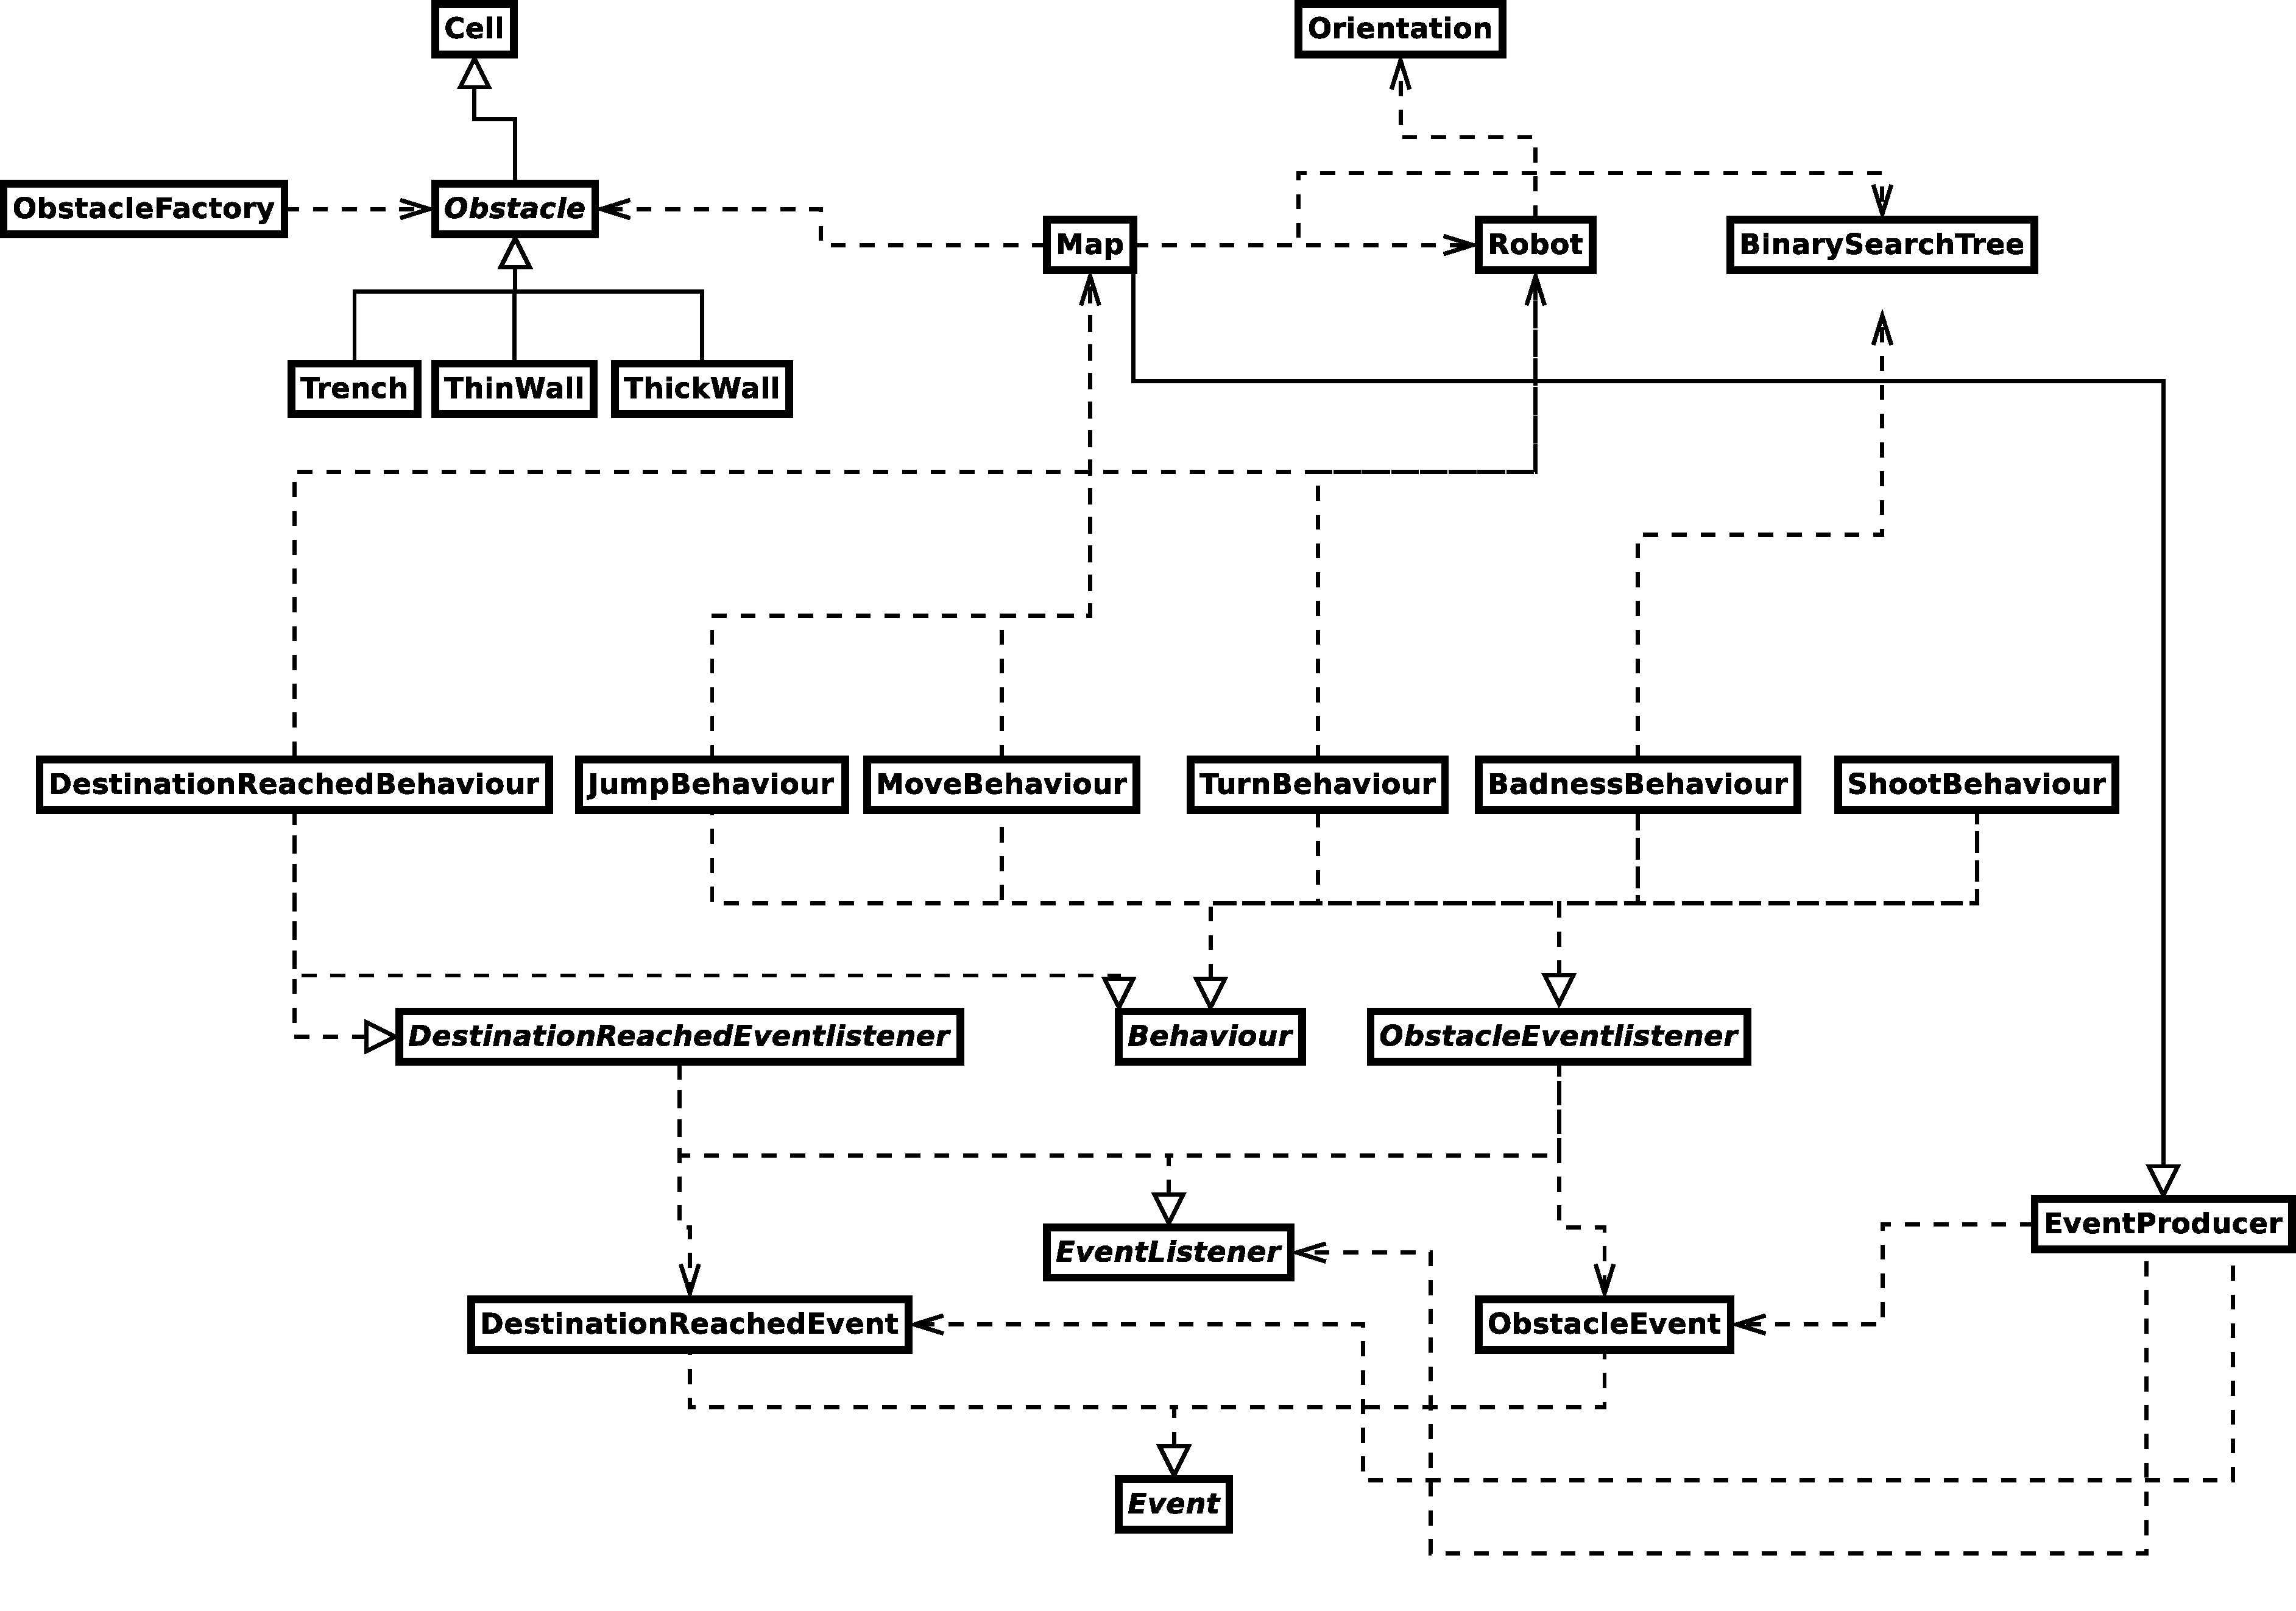
\includegraphics[width=\textwidth]{diagram.pdf}
\caption{Een diagram dat de klassestructuur van het programma toont.}
\label{fig:diagram}
\end{center}
\end{figure}

\subsection*{BadnessBehaviour}
BadnessBehaviour is bad.
\end{document}
